\documentclass[12pt,letterpaper]{article}
\usepackage{fullpage}
\usepackage{wrapfig}
\usepackage{graphicx}
\usepackage{amsmath,amssymb}

\newcommand{\probnumber}[1]{\vspace{2em}\noindent\textbf{(#1)}}

\newcommand{\SE}{{\mbox{SE}}}
\newcommand{\ch}[2]{{{}_{#1}C_{#2}}}
\newcommand{\prob}{{\mbox{Pr}}}
\newcommand{\wt}{\widetilde}
\renewcommand{\SS}{{\mbox{SS}}}
\newcommand{\MS}{{\mbox{MS}}}
\newcommand{\df}{{\mbox{df}}}
\renewcommand{\P}{\mathbb{P}}


\newif{\ifanswers}
% \answerstrue
\answersfalse

\newcommand{\answer}[1]{{\ifanswers \textsf{#1} \else {} \fi}}

\begin{document}


Write the name of an appropriate statistical procedure for the following situations --
for instance ``Wilcoxon--Mann--Whitney test'' or ``chi-squared for goodness of fit'' or ``$t$-test for difference in means''.
\begin{enumerate}
        \renewcommand{\theenumi}{\textbf{\Alph{enumi}}}

    \item We have measured amount of body fat in random samples of male and female elephant seals from three different breeding grounds.  Does the mean amount of body fat differ across breeding grounds, after accounting for differences in the sexes?

      \answer{F-test for two-way ANOVA; just ``ANOVA'' almost correct}
      \ifanswers \else \vspace{\baselineskip} \fi

    \item We have measured people's heights in a random sample; 
      do men and women differ in (population) average height?

        \answer{two--sample $t$-test, or Wilcoxon--Mann--Whitney}
      \ifanswers \else \vspace{\baselineskip} \fi

    \item We have recorded incomes in a random sample of 10 female and 10 male Angelenos;
      do men and women differ in (LA population) average income?
      The distribution of incomes is strongly skewed to the right (i.e.\ has a few values much larger than the others).

      \answer{Wilcoxon--Mann--Whitney; partial credit for two--sample $t$-test}
      \ifanswers \else \vspace{\baselineskip} \fi

%     \item We have measured the average flying speeds in five groups of 20 flies;
%         each group was given a different number of milligrams of caffeine in their food.
%         How much does the average flying speed increase, per milligram of caffeine?
%         
%         \answer{$t$-test for no linear correlation/$r=0$/slope $b_1=0$}
%       \ifanswers \else \vspace{\baselineskip} \fi

    \item In a random sample of tumors we have counted the number that fall into three histological grades, which we previously predicted should occur in the ratio 4:2:1.  Are our data consistent with this?

      \answer{chi-squared (for single-sample proportions)}
      \ifanswers \else \vspace{\baselineskip} \fi


\end{enumerate}



\vspace{3em}
\hrule
\vspace{3em}

Here are several statements from academic studies.
What more would you like to know to judge the strength of the statistical evidence
and the importance of the results?

\begin{itemize}

\item ``We pit luna moths against big brown bats [...].  Moth tails lured bat attacks to these wing regions during 55\% of interactions between bats and intact luna moths.''

\answer{sample size, p-value?}

\item ``We observed significant improvement in memory task performance under drug treatment relative to placebo in the aMCI cohorts at the 62.5 and 125 mg BID doses of levetiracetam.''

\answer{how big was the effect?}

\item ``For each root, the force at the time of fracture was recorded in Newtons.  The fracture values of three experimental and negative control groups were significantly higher than the positive control group.''

\answer{how big was the effect?}

\item ``The study also found that young adults with schizophrenia who abused cannabis as teens performed about 26 percent more poorly on memory tests than young adults with schizophrenia who never abused cannabis.''

\answer{$P$-value? sample size?}


\end{itemize}


\vspace{3em}
\hrule
\vspace{3em}

% two-sample, quantitative data:
% report effect size
% do t-test for mean zero
% discuss confounding factors
\begin{wrapfigure}{r}{2in}
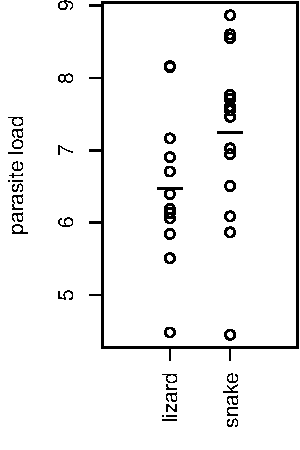
\includegraphics{final-t-test}
\vspace{-1in}
\end{wrapfigure}
We are interested in whether a certain parasite prefers some species over others,
and so have measured parasite load (mg of parasite per animal) 
in random samples of 12 fence lizards and 15 garter snakes in the same habitat,
finding that the average load in lizards is 6.474, with an SD of 1.047,
and the average load in snakes is 7.247, with an SD of 1.161.
The data are shown on the right.
\begin{enumerate}
        \renewcommand{\theenumi}{\textbf{\Alph{enumi}}}
  \item Estimate the effect size of the difference in average load,
      assuming the population SDs are equal to 1.0 for both lizards and snakes,
      and briefly say what it means, in words.

      \answer{
      Effect size is
      \[ \frac{7.247-6.474}{1.0} = 0.773 , \]
      i.e.\ the difference between the samples is about 3/4th of the SD of the variation within samples.
      }
      % \vspace{8\baselineskip}

  \item State an appropriate null and alternative hypothesis for a two--sample $t$ test of the difference in means.

    \answer{
    \begin{align*}
      H_0 : \mu_{\text{lizards}} = \mu_{\text{snakes}}; \quad \text{population mean load is the same for each} \\
      H_A : \mu_{\text{lizards}} \neq \mu_{\text{snakes}}; \quad \text{population mean load differs}
    \end{align*}
    }
      % \vspace{5\baselineskip}

  \item Carry out the $t$ test of these hypotheses, with $\alpha=0.05$.

    \answer{
    \begin{align*}
      \SE_{\bar Y_1 - \bar Y_2} &= \sqrt{ \frac{ 1.047 }{ 12 } + \frac{ 1.161 }{15} } = 0.4057709 \\
      df &= \frac{ (1.047^2 + 1.161^2 )^2 }{ 1.047^4 / 11  + 1.161^4 / 14 } = 24.99266 \\
      t_s &= \frac{0.773}{0.4057709} = 1.905016 \\
      .06 < P &< .08 
   \end{align*}
    }
    % \vspace{7\baselineskip}

  \item What can we conclude about whether the parasite prefers snakes or lizards?

    \answer{
       We have weak evidence that there is a difference in parasite load,
          but would need a larger sample size to find out more confidently.
          }


\end{enumerate}

\vspace{3em}
\hrule
\vspace{3em}


% paired-sample comparisons with zeros
% do sign test
% estimate probability that comparison is +
% and give CI
% why is it better to do sign test than chi-squared for proportions?
We hypothesize that students feel better on Mondays than on Fridays, thanks to having more time for sleep.
A randomly chosen group of 40 USC students reported their general mood on a Monday and the following Friday.  
Of these, 26 reported having a better mood on Monday,
and 14 reported having a better mood on  Friday.
\begin{enumerate}
        \renewcommand{\theenumi}{\textbf{\Alph{enumi}}}
  \item State the null and alternative hypotheses, in words and then in symbols.

    \answer{
    \begin{align*}
      H_0 &: \P\{ \text{mood better on Monday} \} = \P\{ \text{mood better on Friday} \}, \\
      &\text{ students were just as likely to be in a better mood on Monday or on Friday } \\
      H_A &: \P\{ \text{mood better on Monday} \} > \P\{ \text{mood better on Friday} \}, \\
      &\text{ students were more likely to be in a better mood on Mondays. }
    \end{align*}
    }
    % \vspace{5\baselineskip}

  \item Test the null hypothesis using a sign test, and briefly state your conclusion.

    \answer{
      $D = 12$, $n_d=40$, $.0005 < P < .006$.
      We have strong evidence students are more likely to be in a better mood on Mondays (but, we don't know why).
    }
    % \vspace{8\baselineskip}

  \item Estimate the proportion of USC students that feel better on Mondays than on Fridays, and give a 95\% confidence interval for this proportion.

    \answer{
    Wilson's estimator is: 
    \begin{align*}
    \tilde p &= 28/44 = 0.6363636, \\
    \SE_{\tilde P} &= \sqrt{ 0.6363636(1-0.6363636) / 44 } = 0.07252037 \\
    \end{align*}
    so a 95\% CI is $0.6363636 \pm 1.96 \times 0.07252037 = (0.4942237, 0.7785035)$.
    }
    % \vspace{7\baselineskip}

  \item Suppose we could not look up the $P$-value for the sign test on the table,
      but do have 40 fair coins.
      Briefly describe how we could use those coins to estimate the $P$-value in part B.
      \emph{(this should take less than three sentences)}

      \answer{
      Flip all 40 coins and write down the difference in number of heads and number of tails.  Repeat this many times.  The $P$ value is estimated by the fraction of the times that we see at least 12 more heads than tails.
      }

\end{enumerate}



\vspace{3em}
\hrule
\vspace{3em}

Suppose we have incomes (in dollars per year) from ten randomly sampled wife-husband pairs of LA residents:
\begin{center}
\begin{tabular}{r|rrrrrrrrrr}
  \hline
    wife     &  14000  &  17000  &  15000  &  35000  &  84000  &      0  &  19000  &  48000  &   23000  &  11000  \\
    husband  &  24000  &  17000  &  35000  &      0  &  98000  &  15000  &  12000  &  20000  &  196000  &  21000  \\
  \hline
\end{tabular}
\end{center}
We would like to know if, in married heterosexual couples in LA, whether one gender tends to earn more money than the other.

\begin{enumerate}

    \item Give two reasons why the Wilcoxon Signed-Rank test is a good choice for these data.

        \answer{paired samples; very skewed data.}

    \item State the null and alternative hypotheses appropriate for carrying out a Wilcoxon Signed-Rank test.

    \item Carry out the Wilcoxon Signed-Rank test.

    \item What can we conclude about whether LA wives or husbands tend to have larger incomes?

\end{enumerate}


\end{document}


\vspace{3em}
\hrule
\vspace{3em}

% numerical data in categories
% find SS, MS
% do F-test for mean effects
% interpret
To study whether summer daylength causes human hair to absorb more light,
we measured hair absorbance (larger numbers mean more absorbance) in random samples from four cities at different latitudes in Europe, summarized here:
\begin{center}
\begin{tabular}{lrrrr}
  \hline
 & Barcelona & London & Paris & Stockholm \\ 
  \hline
mean & 4.41 & 5.04 & 4.73 & 5.52 \\ 
  SD & 0.84 & 0.71 & 0.90 & 0.87 \\ 
  n & 12 & 10 & 20 & 9 \\ 
   \hline
\end{tabular}
\end{center}

\begin{enumerate}
        \renewcommand{\theenumi}{\textbf{\Alph{enumi}}}
  \item State the null hypothesis in words, and then in symbols.

    \answer{
    \begin{align*}
      H_0 &: 
      \text{mean hair absorbance is the same in all cities} \\
&\mu_{\text{Barcelona}} = \mu_{\text{London}} = \mu_{\text{Paris}} = \mu_{\text{Stockholm}} \\
    \end{align*}
    }
    % \vspace{7\baselineskip}

  \item Construct the ANOVA table and test the null hypothesis.

    \answer{
    \begin{align*}
      \bar{\bar y} &= \frac{ 12 \times 4.41 +  10 \times 5.04 + 20 \times 4.73 + 9 \times 5.52 }{ 51 } = 4.854902 \\
      \SS(\text{within}) &= 11 \times 0.84^2 + 9 \times 0.71^2 + 19 \times0.90^2 + 8 \times 0.87^2 = 27.80723 \\
      \df(\text{within}) &= 47 \\
      \MS(\text{within}) &= 0.5916432 \\
      \SS(\text{between}) &= 12 \times 0.444902^2 + 10 \times 0.185098^2 20 \times + 0.124902^2 + 9 \times 0.665098^2 \\
      \df(\text{between}) &= 3 \\
      \MS(\text{between}) &= 0.2300516
    \end{align*}
    $F_s = 0.2300516/0.5916432 = 0.388835$, so $P>.2$.
    Fail to reject the $H_0$.
    }
    % \vspace{7\baselineskip}

  \item Estimate the within-group variability with the pooled standard deviation.

    \answer{
    \[
    s_\text{pooled} = \sqrt{ \frac{ 11 \times 0.84^2 + 9 \times 0.71^2 + 19 \times .9^2 + 8 \times .87^2  }{ 47 } } = 0.8473199 ,
    \]
    }
    % \vspace{7\baselineskip}

  \item Assess the strength of the evidence for and against the alternative hypothesis (i.e.\ what can we conclude).

  \answer{
  We didn't find any evidence of a relationship between latitude and hair absorbance;
  however, there are confounding factors (genetics).
  Since the effect size we see is comparable to the within-group variability,
  we'd need much larger sample sizes, in any case.
  }

\end{enumerate}

\vspace{3em}
\hrule
\vspace{3em}

% bivariate continuous data, explicit
% formulate hypothesis
% do linear regression
% test for significant effect
\begin{wrapfigure}{r}{3in}
  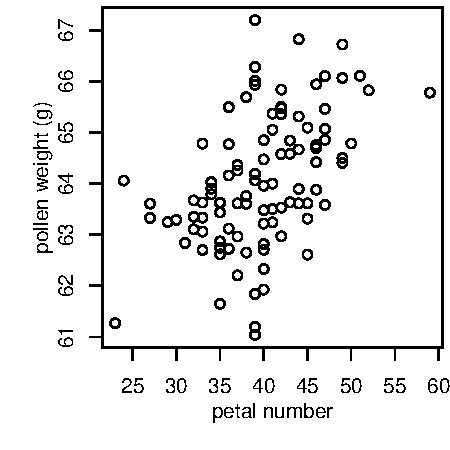
\includegraphics{sunflowers.pdf}
  \vspace{-2in}
\end{wrapfigure}

It is hypothesized that flowers with more petals also produce more pollen.
To test this, we have measured petal number and weight of pollen of 100 sunflowers,
each from different plants,
shown at right.
The mean number of petals is 39.62, with an SD of 6.18;
the mean weight of pollen is 64.05, with an SD of 1.29;
and the correlation between them is $r=0.49$.

\vspace{.85in}

\begin{enumerate}
        \renewcommand{\theenumi}{\textbf{\Alph{enumi}}}
  \item Write the equation for the least-squares regression line,
      and draw this line on the plot.

      \answer{
      Slope is $b_1 = .49 \times 1.29 / 6.18 = 0.1022816$; intercept is $b_0 = 64.05-0.1022816\times39.62 = 59.9976$.
      \[
      \text{(pollen weight)} = 0.1022816 \text{(petal number)} + 59.9976 .
      \]
      }
    % \vspace{6\baselineskip}

  \item Formulate null and alternative hypotheses appropriate for a test of a linear relationship in words, and then in symbols.

    \answer{
    \begin{align*}
      H_0 &: \text{there is not a linear relationship between average petal number and average pollen weight} \\
      & b_1 = 0 \\
      H_A &: \text{there is a linear relationship between average petal number and average pollen weight} \\
      & b_1 \neq 0 
    \end{align*}
    }
    % \vspace{5\baselineskip}

  \item Test the null hypothesis, and briefly state the conclusions.

    \answer{
      \begin{align*}
        t_s &= .49 \sqrt{ \frac{ 98 }{ 1-.49^2 } } = 5.564561 \\
        df &= 98
      \end{align*}
      and $P<.001$;
      we have strong evidence of a linear relationship between mean petal number and mean pollen weight.
    }
    % \vspace{7\baselineskip}

  \item If we found out that our field assistants had cut corners by collecting many of the sunflowers from the same plant, 
      would this call our conclusions into question? 
      Explain, briefly.

      \answer{
      Yes, because the samples are not independent (flowers from the same plant could be correlated), so we might be overly confident in our results.
      }
\end{enumerate}



